\documentclass[executivepaper]{article}

\usepackage{graphicx}
\usepackage[utf8]{inputenc}
\usepackage[T1]{fontenc}
\usepackage[spanish]{babel}
\usepackage{csquotes}
\usepackage{graphicx}
\usepackage{listings}
\usepackage{xcolor}
\usepackage{hyperref}
\usepackage[left=1.00cm, right=1.00cm, top=2.00cm, bottom=2.00cm]{geometry}
\usepackage{tikz}
\usetikzlibrary{shapes,arrows}
\usetikzlibrary{positioning}
\setlength{\parindent}{0.5in}
\usepackage{setspace}
\doublespacing

\lstdefinelanguage{JavaScriptReactHTML}{
  keywords={typeof, new, true, false, catch, function, return, null, catch, switch, var, if, in, while, do, else, case, break},
  keywordstyle=\color{blue}\bfseries,
  ndkeywords={class, export, boolean, throw, implements, import, this},
  ndkeywordstyle=\color{darkgray}\bfseries,
  identifierstyle=\color{black},
  sensitive=false,
  comment=[l]{//},
  morecomment=[s]{/*}{*/},
  commentstyle=\color{purple}\ttfamily,
  stringstyle=\color{red}\ttfamily,
  morestring=[b]',
  morestring=[b]",
  morekeywords={[2]{useState, useEffect, render, Component, props, state, let, const, default, extends}},
  keywordstyle={[2]\color{purple}\bfseries},
  morekeywords={[3]{div, span, input, button, form, h1, App}},
  keywordstyle={[3]\color{teal}\bfseries},
}

\lstset{
    basicstyle=\ttfamily,
    language=JavaScriptReactHTML,
    backgroundcolor=\color{lightgray},
    extendedchars=true,
    basicstyle=\footnotesize\ttfamily,
    showstringspaces=false,
    showspaces=false,
    numbers=left,
    numberstyle=\footnotesize,
    numbersep=9pt,
    tabsize=2,
    breaklines=true,
    showtabs=false,
    captionpos=b,
    literate={~} {$\sim$}{1}
}

\lstdefinestyle{mystyle}{
    backgroundcolor=\color{backcolour},   
    commentstyle=\color{codegreen},
    keywordstyle=\color{magenta},
    numberstyle=\tiny\color{codegray},
    stringstyle=\color{codepurple},
    basicstyle=\ttfamily\footnotesize,
    breakatwhitespace=false,         
    breaklines=true,                 
    captionpos=b,                    
    keepspaces=true,                 
    numbers=left,                    
    numbersep=5pt,                  
    showspaces=false,                
    showstringspaces=false,
    showtabs=false,                  
    tabsize=2
}

\lstset{style=mystyle}

\definecolor{codegreen}{rgb}{0,0.6,0}
\definecolor{codegray}{rgb}{0.5,0.5,0.5}
\definecolor{codepurple}{rgb}{0.58,0,0.82}
\definecolor{backcolour}{rgb}{0.95,0.95,0.92}

\hypersetup{
    colorlinks=true,
    linkcolor=black,
    filecolor=magenta,      
    urlcolor=gray,
}

\title{Arquitecturas para aplicaciones React y patrones de diseño}
\author{Kevin Cárdenas}

\begin{document}

\begin{titlepage}
    \begin{center}
        {\Huge \textbf{Arquitecturas para aplicaciones React y patrones de diseño}}
        \\[17cm]

        \large\emph{Autor:}\\
        Kevin Cárdenas.
        \\[1cm]
        {\large 2024}
    \end{center}
\end{titlepage}

\newpage
\tableofcontents
\newpage

\section{Patrones de diseño}

Los patrones de diseño son soluciones probadas para problemas comunes en el desarrollo de software. En el contexto de React, existen varios patrones de diseño que se utilizan para estructurar y organizar aplicaciones React de manera eficiente y sostenible.

\subsection{Reducer}

Reducer es un patron de diseño que se utiliza para manejar el estado de una aplicación. En el contexto de React, un reducer es una función que toma el estado actual y una acción, y devuelve un nuevo estado. Los reducers son comunes en aplicaciones basadas en Redux, una biblioteca de gestión de estado para aplicaciones JavaScript o Typescript.

La idea principal detrás de los reducers es que permiten manejar el estado de una manera predecible y escalable. Al dividir el estado en piezas más pequeñas y manejar las actualizaciones a través de acciones, los reducers pueden simplificar la lógica de la aplicación y facilitar el mantenimiento.

Para nuestra Arquitetura tendremos 5 modulos principales:

\begin{itemize}
  \item \textbf{Models} (Modelos): Contiene la definición de los datos, un modelo en este caso es un objeto que representa una entidad de la aplicación, como un usuario, un producto, una publicación, etc. No necesitan pruebas unitarias.
  \item \textbf{Services:} (Servicios): Contiene servicios transparentes con el backend, estos servicios se encargan de realizar peticiones HTTP, usualmene no contienen lógica de negocio, y tampoco utilidades. No necesitan pruebas unitarias.
  \item \textbf{Context:} (Contexto): Contiene el contexto de la aplicación, es decir, el estado global de la aplicación, y las acciones que pueden modificar ese estado. Necesitan pruebas unitarias, pero es puramente funcional (.ts o .js).
  \item \textbf{Reducers:} (Reductores): Contiene los reductores, que son funciones puras que toman el estado actual y una acción, y devuelven un nuevo estado. Necesitan pruebas unitarias, pero es puramente funcional (.ts o .js).
  \item \textbf{UI:} (Interfaz de Usuario): Contiene los componentes de la interfaz de usuario, estos componentes se encargan de mostrar la información y de manejar la interacción del usuario. Necesitan pruebas unitarias, en este caso no es puramente funcional (.tsx o .jsx).
  \item \textbf{App:} (Aplicación): Contiene el punto de entrada de la aplicación, y se encarga de inicializar el contexto y renderizar la interfaz de usuario.
\end{itemize}

El patrón de diseño de reductor es especialmente útil para manejar el estado global de una aplicación, ya que permite dividir la lógica de la aplicación en piezas más pequeñas y manejar las actualizaciones de estado de manera predecible y escalable.

En este diagrama se muestra el flujo de la arquitectura con el patrón de diseño de Reducer. La aplicación comienza en el punto de entrada, donde se inicializa el contexto y se renderiza la interfaz de usuario. Los componentes de la interfaz de usuario interactúan con el contexto para leer y actualizar el estado global de la aplicación. Los reductores manejan las actualizaciones de estado en respuesta a las acciones, y los servicios se encargan de realizar peticiones al backend. Los modelos definen la estructura de los datos que se utilizan en la aplicación.

\begin{figure}
  \begin{center}
    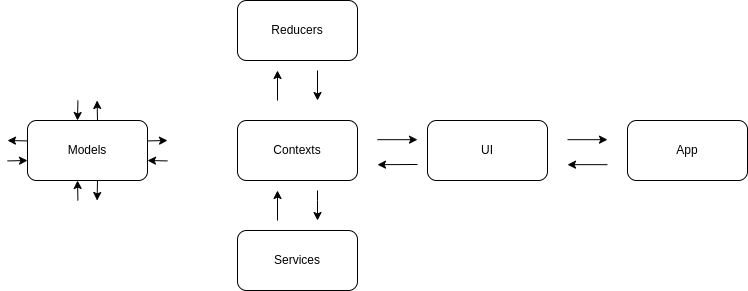
\includegraphics[width=0.7\textwidth]{diagrama_flujo_reducer.png}
    \caption{Diagrama de flujo de la arquitectura con el patrón de diseño de Reducer}
  \end{center}
\end{figure}

\end{document}
